\textbf{\section{Power Analysis} \label{sec:power_analysis}}

% TO DO - SCALE 

\begin{center}
\begin{table} [h!]
\centering
\resizebox{\columnwidth}{!}{ % TO DO- table scale
\begin{tabular}{ |c|c|c|c|c|c| } 
\hline
Component & Average Idle Current (A) & Average Idle Power (W) & Max Current (A) & Max Power (W) \\
\hline
Raspberry Pi Zero WH & 0.18 & 0.9 & 0.42 & 2.1\\
\hline
Arduino Uno R3 & 0.04 & 0.17 & 0.07 & 0.297 \\
\hline
Servo Motor & 0.03 & 0.1275 & 0.22 & 0.935\\
\hline
\end{tabular}}
\caption{Power Analysis of the Project}
\label{table:power_analysis}
\end{table}
\end{center}

The Table~\ref{table:power_analysis} shows the power consumption under idle and maximum cases. The value of the idle case is the average over 20 minute measurement. The maximum case occurs while the camera is working. Power distribution diagram is shown in Figure~\ref{fig:powerdist}. 

    Weight sensor and sonar sensors and analog to digital converter are supplied from the raspberry pi since they do not require high current. 

    Battery unit one shown in Figure 12 contains two Li-Ion batteries connected in series, which supplies 7.4 V to the servo motor. The idle current of this unit is 0.03 A, and the maximum current that occurs during the rotation is 0.22 A. The maximum current occurs for 0.2s, and then it returns to its idle case. The lithium-ion batteries used in this unit have 2000mAh capacity. This unit can operate for 90 hours on the batteries at its maximum power-consuming operation according to mathematical calculations. However, this time is not tested in the system, and it will be less than 90 hours due to the efficiency of the batteries. But, the real-time will be higher than 5 hours. Thus the requirement about the operating time of 5 hours is satisfied.
        
    
    
    Battery unit two shown in Figure 12 contains two Li-Ion Batteries that have 2650mAh capacity connected in parallel. Hence, the overall battery capacity is 5300mAh, and the unit supplies both Raspberry Pi and Arduino Uno. Raspberry pi draws 0.18 A average on the idle case and 0.42 A on the maximum case. The maximum case occurs when the camera module is activated. Also, Arduino draws 0.04 amperes average on the idle case and 0.07 A on the maximum case. Hence, the maximum current driven from the supply is 0.49A, and the system is able to operate on the batteries for at least 10 hours. Therefore, the requirement for operation time is satisfied.    
    
    

\begin{figure}[ht]
     \centering
     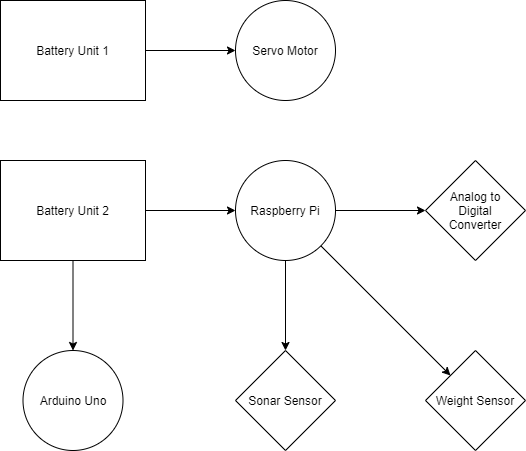
\includegraphics[width=0.75\linewidth]{content/150_power_analysis/powerdiagram.png}
     \caption{ Power Distribution Diagram of the Project}
     \label{fig:powerdist}
\end{figure}